\documentclass[10pt]{beamer}

\mode<presentation>
{
  \usetheme[height=1.25cm]{Madrid}
  \setbeamertemplate{navigation symbols}{}
  \setbeamercolor{alerted text}{fg=illini}
}
\usebackgroundtemplate{
\includegraphics[width=\paperwidth,height=\paperheight]{uc-background}}

\usepackage[english]{babel}
\usepackage{epsfig,subfigure,bm}
\usepackage{multimedia}
\usepackage{psfrag}
\usepackage{animate}

%%%%%% Begin of my macros and options

\setbeamertemplate{section in toc shaded}[default][55]
\setbeamertemplate{subsection in toc shaded}[default][55]
\setbeamercolor{block title}{fg=white,bg=illini}
\setbeamercolor{block body}{fg=black,bg=mygrey}

\setbeamercolor{emphprimary}{fg=CBlue}
\setbeamercolor{emphsecondary}{fg=illini}
\setbeamercolor{emphtertiary}{fg=mygreen}
\definecolor{darkForestGreen}{rgb}{.1,1,.1}
\definecolor{veryLightGray}{rgb}{.9,.9,.9}
\definecolor{greenApple}{rgb}{.3,.9,.3}

\setbeamercolor{frametitle}{bg=CBlue}   
\setbeamercolor{title}{bg=CBlue}

\usepackage{amsmath,amssymb,amsxtra,amsthm}
\usepackage{algorithm,algorithmic}
\usepackage{natbib}
\usepackage{bibentry}
\usepackage{xspace}
\usepackage{changepage}

\pdfmapfile{+sansmathaccent.map}

\definecolor{myblue}{rgb}{.2,.2,.7}
\definecolor{myred}{rgb}{.7,.2,.2}
\definecolor{mygreen}{rgb}{.2,.7,.2}
\definecolor{mygrey}{rgb}{0.9,0.9,0.9}
\definecolor{CBlue}{cmyk}{1,0.25,0,0}
\definecolor{illini}{rgb}{0.98,0.4,0.05}
\definecolor{black}{cmyk}{0,0,0,1}

\newcommand{\myemph}[1]{{\usebeamercolor[fg]{emphprimary}
    \textbf{#1}}}
\newcommand{\myemphalt}[1]{{\usebeamercolor[fg]{emphsecondary}
    \textbf{#1}}}

\graphicspath{{figs/}}

\title[Lecture 1] % (optional, use only with long paper titles)
{CSE276C - Mathematics for Robotics}

\author[H.I. Christensen] % (optional, use only with lots of authors)
{Henrik I.~Christensen}
% - Give the names in the same order as the appear in the paper.  -
% Use the \inst{?} command only if the authors have different
% affiliation.

\institute[UCSD] % (optional, but mostly needed)
{
  \begin{minipage}[c]{.2\textwidth}
    
\includegraphics[width=.65\linewidth]{ucsealnew}%
  \end{minipage}%
  \begin{minipage}[c]{.6\textwidth}
    \small
%%    \begin{center}
      Computer Science and Engineering\\
      University of California, San Diego\\
      \myemph{\url{http://cri.ucsd.edu}}\\          
%%    \end{center}

  \end{minipage}
%%  \vspace*{1ex}
}
%% - Use the \inst command only if there are several affiliations.
%% - Keep it simple, no one is interested in your street address.

\bigskip

\date[Oct 2020]% (optional, should be abbreviation of conference name)
{\small%
  October 2020}

\begin{document}
  
\nobibliography{/Users/hic/Dropbox/bibliography/bib-file}
\bibliographystyle{plain}

\begin{frame}[plain]
  \titlepage
\end{frame}

\begin{frame}
  \frametitle{Introduction}
  \begin{itemize}
    \item Lecturer
    \item Structure
    \item Materials
    \item Information Sources
    \item Transformations
  \end{itemize}
\end{frame}

\begin{frame} 
  \frametitle{Henrik I Christensen}
  \begin{itemize}
    \item Professor at UCSD 
    \item Director of Robotics 
    \item ``Real Systems for Real Problems''
    \item Multi-Robot coordination
    \item Autonomous Driving Vehicles
    \item First commercial robot vacuum cleaner
    \item Working with Boeing, GM, Qualcomm, Robust.AI, ... 
  \end{itemize}
\end{frame} 

\section{Introdution}

\begin{frame}
  \frametitle{Structure of course}
  \begin{columns}
    \column{5cm}
    \begin{itemize}
    \item Lectures
    \item Homework
    \item Discussions      
    \end{itemize}\pause
    \column{5cm}
    \begin{itemize}
    \item Linear Systems
    \item Subspace Methods
    \item Optimization
    \item Root Finding
    \item Integration
    \item Differential Geometry
    \item Space \& Search
    \end{itemize}
  \end{columns}
\end{frame}

\begin{frame}
  \frametitle{Objectives}
  \begin{itemize}
  \item Basic tools for study of robotics
  \item Core mathematical concepts
  \item A few example applications
  \item What are key tools for perception, planning and basic control
  \end{itemize}
\end{frame}

\begin{frame}
  \frametitle{Textbooks}
  \begin{columns}
    \column{7cm}
    \begin{itemize}
    \item W. H. Press, B. P. Flannery, S. A. Teukolsky, and W. T. Vetterling. ``Numerical Recipes''. Cambridge University Press. (Any edition.)
    \item T. Bewley, Numerical Renaissance: simulation, optimization, \& control
    \item M. Deisenroth, A. Aldo Faisal, and C. Soon Ong, "Mathematics for Machine Learning", Cambridge University Press, 2019
    \end{itemize}
    \column{3cm}
    \begin{center}
      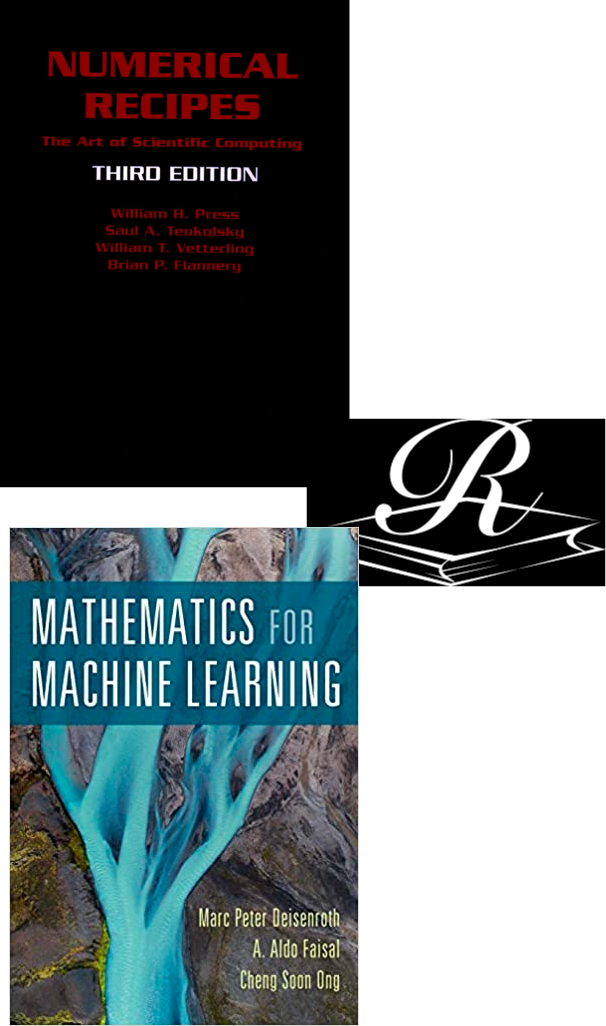
\includegraphics[height=5cm]{books}
    \end{center}
  \end{columns}
\end{frame}

\begin{frame}
  \frametitle{Information Sources}
  \begin{itemize}
  \item CANVAS website
  \item WebSite - http://www.hichristensen.com/CSE276C-20
  \item Piazza - Did you all get an invite?
  \item Office Hours - Henrik \& TA 
  \item Video Lectures available from CANVAS site
  \end{itemize}
\end{frame}

\begin{frame}
  \frametitle{Homework}
  \begin{itemize}
  \item 5 Homework assignments $\approx$ two weeks
  \item Some basic math - analysis by manual or automated
  \item Simple math problems in robotics (could be Python/Numpy or MatLab)
  \item Analysis of sample robotics data
  \end{itemize}
\end{frame}

\begin{frame}
  \centerline{\Huge QUESTIONS?}
\end{frame}

\section{Position and Rotations}

\begin{frame}
  \frametitle{Space and Rotations}
  \begin{itemize}
  \item How do you represent the position of a robot in space?
    \pause 
    \begin{equation*}
      ~^{j}p_{i} = \left( \begin{array}{c} ~^{j}p_{x_i} \\ ~^{j}p_{y_i} \\ ~^{j}p_{z_i}  \end{array} \right)
    \end{equation*}
  \item The position of $i$ with respect to $j$
  \item examples
    \begin{itemize}
    \item World reference frame
    \item Position of the robot
    \item Sensor position or a sensor point
    \end{itemize}
  \end{itemize}
\end{frame}

\begin{frame}
  \frametitle{Example Reference Frames}
  \centerline{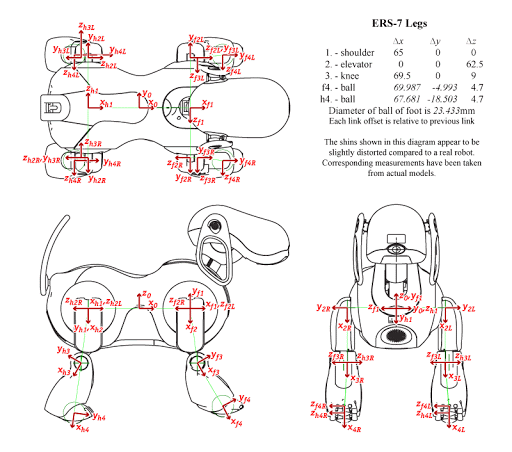
\includegraphics[height=6cm]{sony-trfs}}
\end{frame}
  
\begin{frame}
  \frametitle{Rotation between two reference frames - i, j}
  \[
    ^{j}\mathbf{R}_i = \left(
      \begin{array}{ccc}
        \vec{x}_i \vec{x}_j & \vec{y}_i \vec{x}_j & \vec{z}_i \vec{x}_j \\
        \vec{x}_i \vec{y}_j & \vec{y}_i \vec{y}_j & \vec{z}_i \vec{y}_j \\
        \vec{x}_i \vec{z}_j & \vec{y}_i \vec{z}_j & \vec{z}_i \vec{z}_j \\
      \end{array}
    \right)
  \]
  
  \vspace{1cm}
  \begin{center}
    where $(\vec{x}_i, \vec{y}_i, \vec{z}_i)$ and $(\vec{x}_j, \vec{y}_j, \vec{z}_j)$ are \\
    basis vectors for the two coordinate frames                          
    
  \end{center}
\end{frame}

\begin{frame}
  \frametitle{Elementary Rotations}
  \begin{itemize}
  \item Rotation around Z-axis
    \[
      R_z(\theta) = \left(
        \begin{array}{ccc}
          \cos \theta &  -\sin \theta & 0 \\
          \sin \theta &   \cos \theta & 0 \\
          0           &             0 & 1 \\
        \end{array}
      \right)
    \]
    \pause 
  \item the same for Y and X
    \[
      R_y(\theta) = \left(
        \begin{array}{ccc}
          \cos \theta  &  0 & \sin \theta  \\
          0             &  1 &   0 \\
          - \sin \theta &  0 &   \cos \theta  \\
        \end{array}
      \right)
    \]
    \[
      R_x(\theta) = \left(
        \begin{array}{ccc}
          1 &  0 &   0 \\
          0 & \cos \theta  &  - \sin \theta  \\
          0 & \sin \theta  &    \cos \theta  \\
        \end{array}
      \right)
    \]
  \end{itemize}
\end{frame}

\begin{frame}
  \frametitle{Considerations for rotations}
  \begin{itemize}
  \item We can do combinations
    \[ ~^{k}\mathbf{R}_i = ~^{k}\mathbf{R}_j ~ ^{j}\mathbf{R}_i \]
    \pause
  \item Note the order is important
    \[
     ~^{k}\mathbf{R}_j ~  ^{j}\mathbf{R}_i \neq  ~^{j}\mathbf{R}_i ~ ^{k}\mathbf{R}_j
    \]
  \item The order and reference frames are very important
  \end{itemize}
\end{frame}

\begin{frame}
  \frametitle{Euler Angles}
  \begin{itemize}
  \item We frequently use Euler angles in robotics
    \centerline{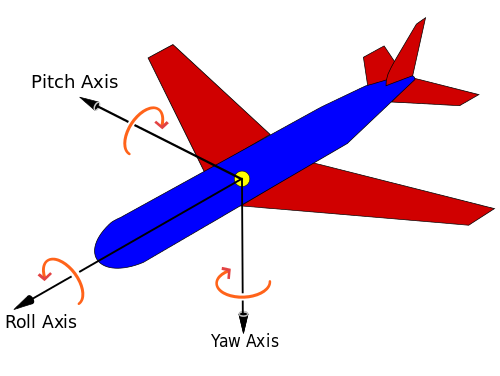
\includegraphics[height=5cm]{euler-angles}}
  \end{itemize}
\end{frame}

\begin{frame}
  \frametitle{Euler Angles}
  \begin{itemize}
  \item The convention used is $R_z R_y R_x$ with respect to $(\alpha, \beta, \gamma)^T$
    \[
      ~^{j}\mathbf{R}_i = \left(
        \begin{array}{ccc}
          c_{\alpha} c_{\beta} & c_{\alpha} s_{\beta} s_{\gamma} - s_{\alpha} c_{\gamma} & c_{\alpha} s_{\beta} c_{\gamma} + s_{\alpha} s_{\gamma} \\
          s_{\alpha} c_{\beta} & s_{\alpha} s_{\beta} s_{\gamma} + c_{\alpha} c_{\gamma} & s_{\alpha} s_{\beta} c_{\gamma} - c_{\alpha} s_{\gamma} \\
          - s_{\beta}          & c_{\beta} s_{\gamma}                                    & c_{\beta} c_{\gamma}\\
        \end{array}
      \right)
    \]
  \end{itemize}
\end{frame}

\begin{frame}
  \frametitle{Derivation of Euler angles}
  \begin{itemize}
  \item If we have the rotation matrix
    \[
      ~^{j}\mathbf{R}_i = \left(
        \begin{array}{ccc}
          r_{11} & r_{12} & r_{13}  \\
          r_{21} & r_{22} & r_{23}  \\
          r_{31} & r_{23} & r_{33}  \\
        \end{array}
      \right)
    \]
  \item derivation of the Euler Angles
    \[
      \begin{array}{cc}
        \beta   & = atan2 \frac{-r_{31}}{\sqrt{r_{11}^2 + r_{21}^2}} \\
        \alpha  & = atan2 \frac{r_{21} / \cos \beta}{r_{11} / \cos \beta}\\
        \gamma  & = atan2 \frac{r_{32} / \cos \beta}{r_{33} / \cos \beta}\\
      \end{array}
    \]
  \end{itemize}
\end{frame}

\begin{frame}
  \frametitle{When may we have problems?}
  \begin{itemize}
  \item Could we have problems? / When?
    \pause
  \item What about singularities?
    \centerline{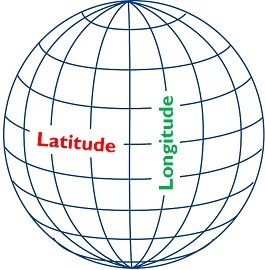
\includegraphics[height=4cm]{lat-long}}
  \end{itemize}
\end{frame}

\begin{frame}
  \centerline{\Huge QUESTIONS?}
\end{frame}


\section{Quaternions}

\begin{frame}
  \frametitle{Quaternions}
  \begin{itemize}
  \item Could we generate a representation that has no singularities?
  \item Hamilton, 1843. 
  \item A 3-parameter family is not adequate (proved by now)
  \item A 4-parameter model is a possibility
  \item Quaternions is a possible representation (not the most intuitive)
  \end{itemize}
\end{frame}

\begin{frame}
  \frametitle{Quaternions}
  \begin{itemize}
  \item Imagine 3-D imaginary numbers - three basis vectors - $\vec{i}, \vec{j}, \vec{k}$
  \item We can represent a quaternion as
    \[
      \vec{\epsilon} = \epsilon_0 + \epsilon_1 \vec{i} + \epsilon_2 \vec{j} + \epsilon_3 \vec{k}
    \]
    or $(\epsilon_0,\vec{\epsilon})$
    \pause
  \item we have three basis vectors
    \[ \vec{i}\vec{i} = \vec{j}\vec{j} = \vec{k}\vec{k} = -1 \]
  \item mixed products
    \[ \vec{i}\vec{j}=\vec{k}, ~ \vec{j}\vec{k} = \vec{i}, ~ \vec{k}\vec{i} = \vec{j}
    \]
    \[
      \vec{j}\vec{i} = -\vec{k}, ~ \vec{k}\vec{j} = -\vec{i}, ~ \vec{i}\vec{k} = -\vec{j}
    \]
  \item Null quaternion
    \[ \vec{0} = 0 + 0\vec{i} + 0 \vec{j} + 0 \vec{k} \]
  \item Unit quarternion
    \[ \vec{1} = 1 + 0 \vec{i} + 0 \vec{j} + 0 \vec{k} \]
  \end{itemize}
\end{frame}

\begin{frame}
  \frametitle{Quaternion operations}
  \begin{itemize}
  \item Product of two quaternions
    \[
      \begin{array}{ccc}
        \vec{a}\vec{b} & = & a_0 b_0 - a_1 b_1-a_2 b_2-a_3 b_3\\
                       & +  & (a_0 b_1 + a_1 b_0 + a_2 b_3 + a_3 b_2 ) \vec{i} \\
                       & +  & (a_0 b_2 + a_2 b_0 + a_3 b_1 - a_1 b_3) \vec{j} \\
                       & +  & (a_0 b_3 + a_3 b_0 + a_1 b_2 - a_2 b_1) \vec{k} \\
      \end{array}
    \]
  \item The good news there are standard libraries
  \end{itemize}
\end{frame}

\begin{frame}
  \frametitle{Rotations w. Quaternions}
  \begin{itemize}
  \item Rotating at an angle $\theta$ around the vector $\vec{a}$ expressed as a quaternion:
    \[
      \vec{\epsilon} = \cos \frac{\theta}{2} + a_x \sin \frac{\theta}{2} \vec{i}
      + a_y \sin \frac{\theta}{2} \vec{j} + a_z \sin \frac{\theta}{2} \vec{k}
    \]    
  \item or
    \[
      \vec{\epsilon} = ( \cos \frac{\theta}{2}, \vec{a} \sin \frac{\theta}{2} )
    \]
  \end{itemize}
\end{frame}

\begin{frame}
  \frametitle{Mapping quaternions to rotation matrices}
  \begin{itemize}
  \item The rotation of a quaternion $\vec{\epsilon}$ can be written as
    \[
      ~^{j}\mathbf{R}_i = \left(
        \begin{array}{ccc}
          1 - 2( \epsilon_2^2 + \epsilon_3^2) & 2 ( \epsilon_1 \epsilon_2 - \epsilon_0 \epsilon_3 ) & 2 ( \epsilon_1 \epsilon_3 + \epsilon_0 \epsilon_2 ) \\
          2 ( \epsilon_1 \epsilon_2 + \epsilon_0 \epsilon_3  ) & 1 - 2 (\epsilon_1^2 + \epsilon_3^2) & 2 ( \epsilon_2 \epsilon_3 - \epsilon_0 \epsilon_1 ) \\
          2 ( \epsilon_1 \epsilon_3 - \epsilon_0 \epsilon_2 ) & 2 ( \epsilon_2 \epsilon_3 + \epsilon_0 \epsilon_1 ) & 1 - 2 (\epsilon_1^2 + \epsilon_2^2) \\
        \end{array} \right)
    \]
  \item As I said the good news there are standard libraries
  \end{itemize}
\end{frame}

\begin{frame}
  \frametitle{From a rotation matrix to quaternions}
  \begin{itemize}
  \item Direct computing the quaternions from a rotation matrix ($\mathbf{R}$)
    \[
      \begin{array}{ccc}
        \epsilon_0 & = & \frac{1}{2} \sqrt{ 1 + r_{11} + r_{22} + r_{33} }\\
        \epsilon_1 & = & \frac{r_{32} - r_{33}}{4 \epsilon_0}\\
        \epsilon_2 & = & \frac{r_{13} - r_{31}}{4 \epsilon_0}\\
        \epsilon_3 & = & \frac{r_{21} - r_{12}}{4 \epsilon_0}\\        
      \end{array}
    \]
  \item Quaternions frequently used in graphics, computer vision and robotics
  \end{itemize}
\end{frame}


\begin{frame}
  \centerline{\Huge QUESTIONS?}
\end{frame}

\section{Homogenous transformations}

\begin{frame}
  \frametitle{Coordinate transformations}
  \begin{itemize}
  \item To move between transformation or move an object we frequently encounter
    \centerline{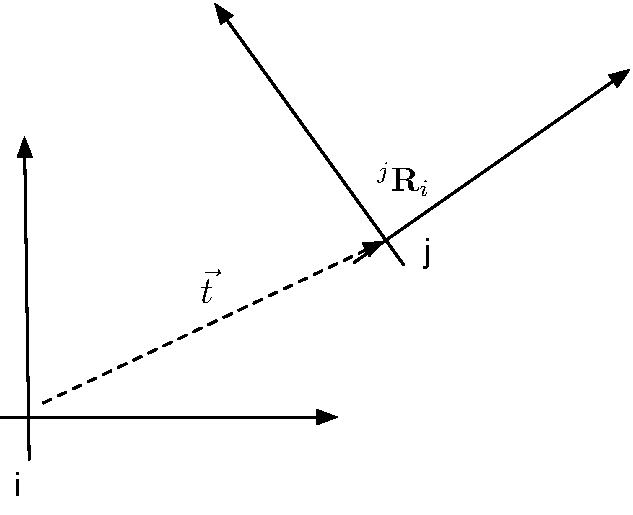
\includegraphics[height=4cm]{geometric-transformation}}
  \item We can write this as $^{j}\vec{p} = ~^{j}\mathbf{R}_i ~^{i}\vec{p} + \vec{t}$
  \end{itemize}
\end{frame}

\begin{frame}
  \frametitle{Homogeneous Transformations}
  \begin{itemize}
  \item We can do this more easily with homogeneous coordinates
    \[
      \vec{P} = \left(
        \begin{array}{c}
          \vec{p} \\ 1 \\
        \end{array}
      \right)
    \]
  \item given this our transformation can now be written as
    \[
      \left(
        \begin{array}{c}
          ^{j}p \\ 1 \\ 
        \end{array}
      \right)
      =
      \left(
        \begin{array}{cc}
          ^{j}\mathbf{R}_i & t \\
          0                & 1 \\          
        \end{array}
      \right)
      \left(
        \begin{array}{c}
          ^{i}p \\ 1 \\ 
        \end{array}
      \right)
    \]
  \item or $ ^{j}P = ~^{j}T_{i} ~~ ^{i}P$

  \end{itemize}
\end{frame}

\begin{frame}
  \frametitle{Standard Joints}
  \begin{itemize}
  \item Revolute joint
    \[
      ^{j}\mathbf{R}_i = \left(
        \begin{array}{ccc}
          \cos \theta & -\sin \theta & 0\\
          \sin \theta & \cos \theta  & 0\\
          0 & 0 & 1\\
        \end{array}
      \right)
    \]
  \item Prismatic joint
    \[
      T = \left(
        \begin{array}{cccc}
          1 & 0 & 0 & 0 \\
          0 & 1 & 0 & 0 \\
          0 & 0 & 1 & d \\
          0 & 0 & 0 & 1 \\
        \end{array}\right)
      = \left(
        \begin{array}{cc}
          I & \begin{array}{c} 0 \\ 0 \\ d \\ \end{array} \\
          0 & 1 \\
        \end{array} \right)
    \]
  \end{itemize}
\end{frame}

\begin{frame}
  \frametitle{Standard Joints (cont.)}
  \begin{itemize}
  \item Cylindrical
    \[
      T = \left(
        \begin{array}{cc}
          R_{\theta} & \begin{array}{c} 0 \\ 0 \\ d \\ \end{array} \\
          0 & 1 \\
        \end{array} \right)
    \]
  \item Spherical
    \[
      T = \left(
        \begin{array}{cc}
          R_{\alpha,\beta,\gamma} & 0 \\
          0 & 1 \\
        \end{array} \right)
    \]
  \item Most other joints can be constructed from these basic models
  \end{itemize}
\end{frame}

\begin{frame}
  \frametitle{Robot dynamics}
  \begin{itemize}
  \item This is an entire field of its own. 
  \item How can we computer the velocity of a robot? 
  \item If we know a desired velocity, how fast should we turn the wheels? 
  \item In general we will refer to the robot actuators as $q_i$
  \item Forward kinematics
    \[
      v = \Phi \dot{q}
    \]
  \item Inverse kinematics
    \[
      \dot{q} = \Phi^{-1} v
    \]
  \item Not get into the much of the details until we talk about differential geometry (end of course)
  \end{itemize}
\end{frame}

\begin{frame}
  \frametitle{Wrap-up}
  \begin{itemize}
  \item Basic course information
    \begin{itemize}
    \item Books, topics, websites, ...
    \end{itemize}
  \item Introduction to positions, rotations, transformations, ... 
  \item Next time we will talk about linear systems of equations
  \end{itemize}
\end{frame}

\begin{frame}
  \frametitle{Questions}
  \centerline{\Huge Questions}
\end{frame}

\end{document}
%%% Local Variables:
%%% mode: latex
%%% TeX-master: t
%%% End:
